\documentclass[10pt,a4paper,landscape]{article}
\usepackage[utf8]{inputenc}
\usepackage[german]{babel}
\usepackage[T1]{fontenc}
\usepackage{amsmath}
\usepackage{amsfonts}
\usepackage{amssymb}
\usepackage{graphicx}
\usepackage{lmodern}
\usepackage{fourier}
\usepackage{array}
\usepackage{array}
\usepackage{multirow}
\usepackage{xcolor}
\usepackage{tcolorbox}
\usepackage{titlesec}
\usepackage{pdfpages}
\usepackage{pgffor}


\usepackage{multicol}
\setlength{\columnsep}{0.5cm}

\usepackage{extsizes}
\newcommand{\setdocumentfont}{\fontsize{6}{8}\selectfont} 


% Schriftgrößenänderung für Section-Titel
\titleformat{\section}[block]{\normalfont\fontsize{8}{10}\bfseries\textcolor{red}}{\thesection}{1em}{}

\titleformat{\subsection}[block]{\normalfont\fontsize{7}{9}\bfseries}{\thesubsection}{1em}{}

\titleformat{\subsubsection}[block]{\normalfont\fontsize{6}{8}\bfseries}{\thesubsubsection}{1em}{}

\usepackage[left=1cm,right=1.2cm,top=1cm,bottom=1cm]{geometry}

\tcbset{
  sectionbox/.style={
    colframe=blue!50!black,
    colback=blue!5,
    coltitle=blue!20!black,
    fonttitle=\bfseries,
    boxrule=0.5mm,
    rounded corners,
    breakable,
    width=\linewidth,
  }
}

\pagestyle{empty}


\title{shitSheat}
\begin{document}
\setdocumentfont
\begin{multicols}{4}
\noindent

\section{Definitionen für Dumme}

\resizebox{0.2\textwidth}{!}{
\begin{tabular}{l l l}
\textbf{Variable} & \textbf{Definition} & \textbf{Kapitel}\\
\hline
$\overline{x}$ & Arithmetisches Mittel &(6.1) \\
$\overline{x}_w$ & Gewichteter Mittelwert &(6.2) \\
$\overline{x}_G$ & Geometrisches Mittel &(6.4)\\
$\overline{x}_H$ & Harmonisches Mittel &(6.5)\\
$\overline{x}_{\alpha}$ & Getrimmtes &(6.7)\\
$s_x^2, \tilde{s}_x^2$ & Stichprobenvarianz &(6.20)\\
$s_x$ & Standardabweichung &(6.21)\\
$\overline{x}_1, \tilde{s}_{x1}^2$ & Schichtmittelwerte und Schichtvarianzen &(6.23)\\
$\sigma(X)$ & Standardabweichung ZV &(6.27)\\
$g_p, g_m$ & Quantilskoeffizient und Momentenkoeffizient &(6.30)\\
$s_{xy}$ & Kovarianz &(10.1)\\
$r_{xy}$ & Bravais-Pearson &(10.2)\\
$Cov(X,Y)$ & Kovarianz ZV &(10.4)\\
$\rho(X,Y)$ & Korrelation ZV &(10.5)\\
$r_{xy}^{SP}$ & Spearman &(10.8)
\end{tabular}
}

\section{Datenerhebung und Messung}


\subsection{Grundbegriffe}

\begin{itemize}
\item Statistische Einheit, Untersuchungseinheit \\
	(Person oder Objekt untersucht)
\item Grundgesamtheit, Population\\
	(gesamte Gruppe, Bsp. Schüler einer Schule)
\item Teilgesamtheit, Stichprobe\\
	(kleiner Teil vom Ganzen)
\item Merkmal, (Ko-)Variable\\
	(bestimmte Eigenschaft, die man messen will)
\item Merkmalsausprägung \\
	(konkreter Wert vom Merkmal)
\item Merkmalsraum (Zustandsraum)\\
	(alle möglichen Werte, die ein Merkmal annehmen kann)
\item Beobachtung\\
	(gemessene Merkmalsausprägungen zu einem bestimmten Zeitpunkt)
\end{itemize}

\subsection{Skalenniveaus}

\subsubsection*{Nominal}
\begin{itemize}
\item Kategorisierung möglich
\item Gleichheit/Ungleichheit bestimmbar
\item keine Rangordung
\item $a=b \Leftrightarrow f(a)=f(b)$
\item Modus 
\end{itemize}

\subsubsection*{Ordinal}
\begin{itemize}
\item Kategorisierung möglich
\item Rangordnung bestimmbar, linear
\item keine gleichmäßigen Abstände zw. Rängen
\item $a<b \Leftrightarrow f(a)<f(b)$
\item Modus, Median
\end{itemize}

\subsubsection*{Intervall}
\begin{itemize}
\item Kategosierung und Rangordnung möglich
\item Abstände zw. Werten quantifizierbar
\item kein natürlicher Nullpunkt
\item $f(x_1)-f(x_2)=f(x_3)-f(x_4) \Leftrightarrow x_1-x_2=x_3-x_4 $
\item Modus, Median, Mittelwert
\end{itemize}

\subsubsection*{Verhältnis}
\begin{itemize}
\item alle Eigenschaften zuvor
\item natürlicher Nullpunkt
\item Verhältnisse zw. Werten interpretierbar
\item $\frac{f(x_1)}{f(x_2)}=\frac{x_1}{x_2}$
\item Modus, Median, Mittelwert
\end{itemize}

\subsubsection*{Absolut}
\begin{itemize}
\item Häufigkeit, Anzahl
\item keine Transformation
\item Modus, Median, Mittelwert
\end{itemize}

\subsubsection*{Zusammenfassung}

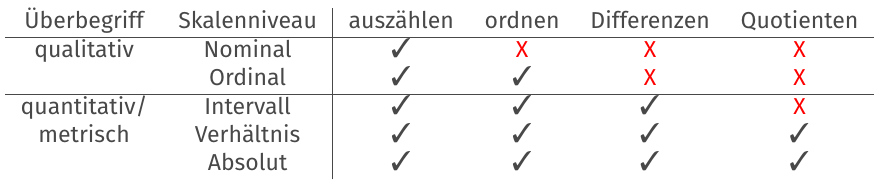
\includegraphics[scale=0.2]{Bilder/Skalen.png} 

\subsection{Merkmalstypen}

\subsubsection*{Diskret}
\begin{itemize}
\item abzählbar
\item keine Zwischenwerte
\item oft ganzzahlig
\end{itemize}

\subsubsection*{Stetig}
\begin{itemize}
\item unendlich viele Ausprägungen
\item Zwischenwerte möglich
\item oft mit Dezimalstellen
\end{itemize}

\subsubsection*{Quasi-Stetig}
\begin{itemize}
\item diskret
\item sehr kleine Einheiten
\item \glqq praktisch\grqq~¨stetig
\end{itemize}

\textcolor{gray}{
\subsubsection*{Gruppierte Daten, Häufigkeitsdaten}
Wertebereich eines (quasi-)stetigen Merkmals in Gruppen eingeteilt\\
Beispiele: Gehalt in Gehaltsklassen, Alter in Altersklassen\\
Gruppierung auch für Datenschutz gut
}

\subsection*{Erhebungsarten}
\begin{enumerate}
\item Umfang
\begin{itemize}
\item Vollerhebung\\
	(alle Stats der gesamten Gruppe)
\item Stichprobe/Teilerhebung\\
	(nur kleiner Teil der gesamten Gruppe untersucht)
\end{itemize}

\item Datenform

\begin{itemize}
\item Querrschnittsdaten\\
	(Momentaufnahme einer Stichprobe)
\item Zeitreihe\\
	(quantitative Auswertung über einen Zeitverlauf)
\item Längsschnittdaten\\
	(Datenerhebung zu versch. Zeitpunkten)
\end{itemize}

\item Methoden operationaler Messungen

\begin{itemize}
\item Beobachtung:\\
verdeckt oder teilnehmend; systematisch mit Beobachtungsprotokoll
\item Befragung: \\
mündlich mit/ohne Interviewer, schriftlich/online, Fragebogen
\item Experiment: \\
kontrollierte Situation, evtl. Erhebung durch Beobachtung oder Befragung
\end{itemize}

\end{enumerate}

%=========================================================================================================================================================================================================================

\section{Statistische Grafiken}

\subsection{grammar of graphics}
\begin{itemize}
\item Daten: Beobachtungen dargestellter Merkmale (Anteile, Mittelwerte, usw.)
\item Geometrische Elemente (Punkte, Linien, Rechtecke, ...)
\item Ästhetische Zuordnung: sichtbare Eigenschaften geom. Elemente (Position, Farbe, Größe, Form)
\item zu vermeiden: Overplotting, zu viele Information in einer Grafik $\rightarrow$ Lsg. Facettierung, Aufteilung in mehrere Grafiken
\end{itemize}

\subsection{Wahrnehmung von Grafiken}
\begin{enumerate}
\item Position (geminsame/parallele Skala > verschobene Skalen)
\item Abstände und Längen 
\item Steigung und Winkel
\item Flächen
\item Volumen
\item Farbton-Farbsättigung-Farbhelligkeit 
\end{enumerate}

\subsection{Farbskalentyp}
\begin{itemize}
\item Qualitativ (variiender Farbton): \\
für nominales Skalenniveau

\item Sequentiell (variiendere Helligkeit): \\
min. ordinales Skalenniveau

\item Divergierend (2 Farben kombiniert): \\
min. ordinales Skalenniveau, mit neutralem Mittelwert
\end{itemize}

\subsection{Visualisierung der Häufigkeiten diskreter Merkmale}
\begin{itemize}
\item Stab-, Säulen-, Balkendiagramm \\
		Anwendungen: Ordinal, Metrisch mit wenig Ausprägungen, Nominal (Problem: bel. Anordnung von Ausprägungen)
\item Stapeldigramm \\
		Anwendungen: Nominal, Ordinal/Gruppiert, Metrisch mit wenig Ausprägungen
\item Kreisdiagramm, Tortendiagramm \\
		Anwendungen: Nominal, Ordianl (Problem: Ordnung nicht korrekt), Gruppiert
\end{itemize}

\subsection{Visualisierung der Häufigkeiten metrischer Merkmale}
\subsubsection{Dotplots}
\begin{itemize}
\item x-Position: Beobachtete Merkmalsausprägungen der UE
\item opt. y-Position: Ausprägungen des bedingenden Merkmals
\item verwendete Geos: Punkte oder anderes
\end{itemize}

\subsubsection{Histogramm}
\begin{itemize}
\item Aufteilung in Klassen
\item Bestimmung von Klassenhäufigkeiten $n_j$ und relativer Häufigkeit $f_j=\frac{n_j}{n}$
\item Histogramm-Höhen $y_j$, sodass $b_j \cdot y_j = f_j$, $b_j$ Breite von Klasse j
\end{itemize}

\subsubsection{Mosaikplots}
\begin{itemize}
\item mehrere diskrete Merkmale dargestellt (Geschlecht, Klasse, Kind/Erwachsen, Überleben)
\item Symmetrie (Fläche gleich groß): Unabhängigkeit, Asymmetrie: Bedingt
\end{itemize}

\subsubsection{Dichtefunktion}
\[
\int_a ^b f(x)dx \approx \frac{1}{n}\mid \lbrace x_i : a < x_i \leqslant b\rbrace \mid
\]

\subsection{Dichte-Kurven}
\begin{align*}
\hat{f}(x) &= \frac{\frac{1}{n}\mid \lbrace x_i : x_i \in [x-h, x+h)\rbrace \mid}{2h} \\
		&= \frac{1}{n} \sum_{i = 1}^n \frac{1}{h}k\left(\frac{x-x_i}{h}\right) \\
		&k(u) = \begin{cases}
    \frac{1}{2}, & \text{für } -1 \leqslant u < 1 \\
    0, & \text{sonst} 
\end{cases}
\end{align*}

Gleitendes Histogramm mit Rechteck-Kernfunktion

\subsection{Kerndichteschätzer}
k(u) sei Kernfunktion, $k(u) \geqslant 0 \forall u$ und K(u) = 1:
\[
\hat{f}(x)= \frac{1}{nh}\sum_{i=1}^n k\left(\frac{x-x_i}{h}\right)
\]
\textbf{Beispiel Kernfunktionen}
\begin{align*}
\text{Gauß-Kern: } &k(u)=\frac{1}{\sqrt{2\pi}}exp\left(-\frac{1}{2}u^2\right) \\
\text{Epanechnikov-Kern: } &k(u)=max(0,\frac{3}{4}(1-u^2)) \\
\text{Dreieck-Kern: } &k(u)=max(0,1- \mid u \mid)
\end{align*}

%=========================================================================================================================================================================================================================

\section{Grundlagen: Wahrscheinlichkeit}

\subsection{Grundbegriffe Stochastik}
\begin{itemize}
\item Ergebnisse $\omega$
\item Menge aller Ergebnisse $\Omega$ (Stochastische Grundgesamtheit)
\item Ereignis $A\subseteq \Omega$
\item Elementarereignis \{$\omega$\}, einziges Ereignis von $\Omega$
\end{itemize}

\subsubsection*{Laplace-Wahrscheinlichkeit}

\[P(A):=\frac{|A|}{|\Omega |}=\frac{|A|}{n}\]

\subsection{Kombinatorik}
\renewcommand{\arraystretch}{0.5} % Erhöht den Zeilenabstand in der Tabelle
\begin{center}
\small % Verkleinert den Text innerhalb der Tabelle
\resizebox{\columnwidth}{!}{%
\begin{tabular}{|c|c|c|}
\hline
 & ohne Zurücklegen & mit Zurücklegen \\
\hline
ohne Reihenfolge & $\binom{n}{k}$ & $\binom{n + k - 1}{k}$ \\
\hline
mit Reihenfolge & $\frac{n!}{(n - k)!}$ & $n^k$ \\
\hline
\end{tabular}%
}
\end{center}

\subsection{Kolmogorov Axiome}
\begin{itemize}
\item Disjunkte Ereigenisse: A, B $\subseteq \Omega$ disjunkt, wenn $A \cap B = \emptyset$
\item Komplement/Gegenereignis: \( \overline{A} := \Omega \setminus A = \{ \omega \in \Omega : \omega \notin A \} \)
\end{itemize}

\subsubsection{Wahrscheinlichkeitsverteilung}
\begin{enumerate}
\item $P(A)\geqslant 0$ für beliebige $A\subseteq \Omega$(Positivität)
\item $P(\Omega )=1$ (Sicheres Ereignis)
\item $P(A \cup B) = P(A) + P(B)$ für disjunkte Ereignisse $A,B \subseteq \Omega$ (Additivität)
\end{enumerate}

\subsubsection*{Wichtiges zur Wahrscheinlichkeitsrechnung}
\begin{itemize}
\item $P(\cup _{i=1} ^{n}) = \sum_{i=1}^n P(A_i)$ für paarweise disjunkte Ereignisse $A_1, A_2, ~..., A_n \subset \Omega$
\item $A \subseteq B \Rightarrow P(A) \leqslant P(B)$
\item \(P (\overline{A}) = 1 - P(A)\)
\item $P(A|\overline{B})= 1 - P(\overline{A} |\overline{B})$
\item $P(\overline{B}\cap A)=P(A|\overline{B})\cdot P(\overline{B})$
\item $P(A\cup B) = P(A) + P(B) -P(A\cap B)$ für beliebige A, B $\subset \Omega$
\end{itemize}

\subsubsection*{Siebformel}
{\tiny
\begin{align*}
P(A_1 \cup A_2 \cup A_3 \cup ... \cup A_n) &= \\
&\sum _{i}P(A_i)- \sum_{i<j}P(A_i \cap A_j)+ \\
&\sum _{i<j<k}P(A_i \cup A_j \cup A_k) \\
P(A \cup B \cup C) \\
&=(P(A)+P(B)+P(C))-(P(A\cap B) + P(A \cap C) \\
&+ P(B\cap C)) + P(A\cap B \cap C)
\end{align*}
}

\textcolor{gray}{\subsubsection*{Bonferroni}
\[ \resizebox{0.25\textwidth}{!}{$
\sum_i P(A_i)\geqslant P(\bigcup_{i=1}^nA_i)\geqslant \sum_i P(A_i) - \sum_{i<j}P(A_i \cup A_j)
$}
\]
}

\subsection{Bedingte Wahrscheinlichkeiten}
\[
P(A|B) := \frac{P(A\cap B)}{P(B)}
\]

\subsubsection*{Eigenschaften}
\begin{itemize}
\item Sicheres Ereignis:
\[
P(B|B) = 1
\]
\item Unmögliches Ereignis:
\[
P(\overline{B}|B) = 0
\]
\item Positivität für beliebige A $\subseteq \Omega$:
\[
P(A|B)\geqslant 0
\]
\end{itemize}

\subsubsection*{Satz der totalen Wahrscheinlichkeit}
\[
P(A)=\sum_{i=1}^n P(A|B_i) \cdot P(B_i)
\]

\subsubsection*{Wichtiger Spezialfall: Multiplikationssatz}
\[
P(A)=P(A|B)P(B)+P(A|\overline{B})P(\overline{B})
\]

\subsection{Stochastische Unabhängigkeit}
\[
P(A|B) = P(A) ~bzw.~ P(B|A)=P(B)
\]
\[
P(A \cap B)=P(A) \cdot P(B)
\]

\subsection{Bedingte Unabhängigkeit}
\[
P(A \cap B|C)=P(A|C)\cdot P(B|C)
\]

\subsection{Satz von Bayes}
\[ \resizebox{0.2\textwidth}{!}{$
P(A|B)=\frac{P(A\cap B)}{P(B)} \Rightarrow P(A\cap B)=P(A|B)P(B)
$}
\]

\[ \resizebox{0.2\textwidth}{!}{$
P(B|A)=\frac{P(B\cap A)}{P(A)} \Rightarrow P(B\cap A)=P(B|A)P(A)
$}
\]

\[
\Rightarrow P(A|B)P(B)=P(B|A)P(A)
\]

\subsection{Satz von Bayes II}
\[ \resizebox{0.2\textwidth}{!}{$
P(B|A)=\frac{P(A|B)P(B)}{P(A)}=\frac{P(A|B)P(B)}{P(A|B)P(B)+P(A|\overline{B})P(\overline{B})}
$}
\]
\[ 
P(B_i|A)=\frac{P(A|B_i)P(B_i)}{\sum_{j=1}^n P(A|B_j)P(B_j)}
\]

\subsubsection*{Wichtiges}
\begin{itemize}
\item $P(A|B)$ Sensitivität (wahr-positiv Rate)
\item $P(\overline{A}|\overline{B})$ Spezifität (wahr-negativ Rate)
\item $P(A)$ Prävalenz
\end{itemize}

\subsection{Odds/Chancen}
Verhältnis von Ergebnis und Gegenergebnis
\subsubsection{Umrechnung Wahrscheinlichkeit in Odds}
\[
\gamma (A):=\frac{P(A)}{1-P(A)}\in [0, \infty]
\]

\subsubsection{Umrechnung Odds in Wahrscheinlichkeit}
\[
P(A)=\frac{\gamma(A)}{1+\gamma(A)}
\]

\subsubsection{Satz von Bayes in Odds-Notation}
\[
\frac{P(B|A)}{P(\overline{B}|A)}=\frac{P(B)}{P(\overline{B})}\cdot \frac{P(A|B)}{P(A|\overline{B})}
\]

\[
\gamma(B|A)=\gamma(B) \cdot \frac{P(A|B)}{P(A|\overline{B})}
\]

\begin{center}
Posterior Odds = Prior Odds $\cdot$ Likelihood Ratio
\end{center}

%=========================================================================================================================================================================================================================

\section{Zusammenhangsmaße diskreter Merkmale}
X = Zeilen \\
Y = Spalten
\subsection{Kontigenztafeln}
\begin{itemize}
\item Absolute Häufigkeit
\[
\begin{array}{c|ccc|c}
  & b_1 & \cdots & b_m & h_{1\cdot} \\
\hline
a_1 & h_{11} & \cdots & h_{1m} & h_{1\cdot} \\
a_2 & h_{21} & \cdots & h_{2m} & h_{2\cdot} \\
\vdots & \vdots & \ddots & \vdots & \vdots \\
a_k & h_{k1} & \cdots & h_{km} & h_{k\cdot} \\
\hline
  & h_{\cdot 1} & \cdots & h_{\cdot m} & n
\end{array}
\]

\item Relative Häufigkeiten
\[
\begin{array}{c|ccc|c}
  & b_1 & \cdots & b_m & h_{1\cdot} \\
\hline
a_1 & f_{11} & \cdots & f_{1m} & f_{1\cdot} \\
a_2 & f_{21} & \cdots & f_{2m} & f_{2\cdot} \\
\vdots & \vdots & \ddots & \vdots & \vdots \\
a_k & f_{k1} & \cdots & f_{km} & f_{k\cdot} \\
\hline
  & f_{\cdot 1} & \cdots & f_{\cdot m} & 1
\end{array}
\]

\end{itemize}

\subsubsection*{Bedingte Häufigkeiten}

\[
f_{Y|X}(b_1|a_1)=\frac{h_{i1}}{h_{i\cdot}},~...,~ f_{Y|X}(b_m|a_i)=\frac{h_{im}}{h{i\cdot}}
\]

\[
f_{X|Y}(a_1|b_1)=\frac{h_{1j}}{h_{\cdot j}},~...,~ f_{X|Y}(a_k|b_j)=\frac{h_{kj}}{h{\cdot j}}
\]

\subsubsection*{Empirisch bedingte Odds}

\[
\gamma (1,2|X=a_i)= \frac{h_{i1}}{h_{i2}}
\]

\subsubsection*{Odds-Ratio}

\[ \resizebox{0.25\textwidth}{!}{$
\gamma (1,2|X=1, X=2)=\frac{\gamma(1,2|X=1)}{\gamma(1,2|X=2)}=\frac{h_{11}/h_{12}}{h_{21}/h_{22}}=\frac{h_{11}h_{22}}{h_{21}h_{12}}
$}
\]

\begin{itemize}
\item $\gamma = 1$ Odds in beiden Subpopulationen gleich
\item $\gamma > 1$ X = 1 größer als X = 2
\item $\gamma < 1$ X = 1 kleiner als X = 2
\end{itemize}

\subsection{Empirische Unabhängigkeit}
\[ \resizebox{0.2\textwidth}{!}{$
f_{Y|X}(b_j|a_1)=f_Y(b_j|a_2)=...=f_{Y|X}(b_j|a_k)\forall j=1,...,m
$}
\]
oder halt:
\[
\forall i,j: ~ h_{ij}=\tilde{h}_{ij}
\]

\subsection{$\chi^2$- und Kontigenzkoeffizient}

\subsubsection*{Berechnung von $\tilde{h}$}
ist erwartete Häufigkeit in einer Kontingenztafel
\[
\text{mit}~~ \tilde{h}_{ij}=\frac{h_{i\cdot}h_{\cdot j}}{n}
\]

\subsubsection*{$\chi^2$-Koeffizient}

{\tiny
\begin{align*}
\chi^2 := \sum_{i=1}^k \sum_{j=1}^m \frac{(h_{ij}-\tilde{h}_{ij})^2}{\tilde{h}_{ij}}&=\sum_{i=1}^k \sum_{j=1}^m \frac{(h_{ij}-\frac{h_{i\cdot}h_{\cdot j}}{n})^2}{\frac{h_{i\cdot}h_{\cdot j}}{n}} \\
&=  n\sum_{i} \sum_{j}\frac{(f_{ij}-f_{i\cdot}f_{\cdot j})^2}{f_{i\cdot}f_{\cdot j}} \\
\text{mit}~~ \tilde{h}_{ij}=\frac{h_{i\cdot}h_{\cdot j}}{n}
\end{align*}
}

\begin{itemize}
\item $\chi^2 \in [0, n(min(k,m)-1)]$
\item $\chi^2=0 \Leftrightarrow$ X und Y empirisch unabhängig
\item $\chi^2$ groß, starker Zusammenhang
\item $\chi^2$ klein, schwacher Zusammenhang
\end{itemize}

\subsubsection*{Spezialfall für 2x2-Tafel}
\[
\begin{array}{|cc|c|}
\hline
a & b & a+b \\
c & d & c+d \\
\hline
a+c & b+d & \\
\hline
\end{array}
\]

\[
\chi^2 = \frac{n(ad-bc)^2}{(a+b)(a+c)(b+d)(c+d)}
\]

\subsubsection*{Kontigenzkoeffizient}
\[ \resizebox{0.25\textwidth}{!}{$
K := \sqrt{\frac{\chi^2}{n+\chi^2}}, ~K \in \left[0, \sqrt{\frac{M-1}{M}}\right],~ M=min\{k, m\}
$}
\]

\subsubsection*{Korrigierter Koeffizient}
\[
K^* := \frac{K}{\sqrt{(M-1)/M}}, ~ K^* \in [0, 1]
\]

%=========================================================================================================================================================================================================================

\section{ZVs, Verteilungen und Häufigkeiten}

\subsection{Zufallsvariable}
\[
X:\Omega \rightarrow T_X , ~ T_X\subseteq \mathbb{R}
\]

\begin{itemize}
\item ordnet jedem $\omega \in \Omega$ genau ein $x \in T_X$ zu: $X(\omega)=x$
\item Mehrere Elementarereignisse können selben Zahlenwert zugeordnet sein
\item Ausprägungen/Relisierungen: $x=X(\omega)$ von X
\end{itemize}

\subsection{Wahrscheinlichkeitsfunktion diskreter ZV}
\[
f(x_i):=P(X=x_i)=P({\omega \in \Omega : x(\omega)=x_i}), ~ x_i \in \mathbb{R}
\]

\[
B\subset \mathbb{R}: ~ P(X \in B) = P({\omega \in \Omega : X(\omega) \in B})
\]

\[
x \notin T: ~ f(x)=P(\emptyset)=0
\]

\subsection{Verteilungsfunktion diskret}
\[
F(x) := P(X\leqslant x) = \sum_{i:x_i\leqslant x} f(x_i)
\]

\textbf{Eigenschaften}
\begin{itemize}
\item monoton wachsend (\glqq Treppenfunktion\grqq)
\item stückweise konstant mit Sprungstellen an $x_i$ mit $f(x_i) > 0$, ~$x_i \in T$
\item Höhe des Sprungs an Stelle $x_i \in T$ ist $f(x_i)$
\item $\lim\limits_{x \to \infty} F(x) = 1$
\item $\lim\limits_{x \to -\infty} F(x)=0$
\end{itemize}

\subsection{Wahrscheinlichkeitsfunktion stetiger ZV}
\[
F(x)=\int_{-\infty}^{X}f(u)du
\]

\textbf{Folgerung}
\begin{itemize}
\item Dichtefunktion ist f(x)
\item $\int_{- \infty}^{+\infty} f(x)dx =1$
\item Teilmenge mit Dichte-/Verteilungsfunktion möglich: $P(X \in [a,b])=\int_a^b f(x)dx= F(b) -F(a)$
\item Unintuitive Konsequenz: $P(X=x)=0 ~\forall x \in \mathbb{R}$
\item $\lim\limits_{x \to \infty} F(x) = 1$
\item $\lim\limits_{x \to -\infty} F(x)=0$
\item $F'(x)=f(x)$, wo $f(x)$ stetig
\item $P(a \leqslant X \leqslant b)=F(b)-F(a)$
\item $P(X>a)= 1-F(a)$
\end{itemize}

\subsection{Empirische Verteilungsfunktion}
Verteilung einer Stichprobe

\[
F_n(x)=\frac{H(x)}{n}
\]
\begin{center}
$\Rightarrow$ Anteil der Werte $x_i$ mit $x_i \leqslant x$\\
Häufigkeitsfunktion: $H(x) :=$ (Anzahl der Werte $\leqslant x$)
\end{center}

\[ \resizebox{0.25\textwidth}{!}{$
F_n(x)=f(a_1)+...+f(a_j)=\sum_{i:a_i \leqslant x} f_i, ~a_j\leqslant x, ~a_{j+1}>x 
$}
\]

\textbf{Eigenschaften ECDF $\mathbf{F_n(x)}$(empirical cumulative distribuation function)}
\begin{itemize}
\item monoton wachsende Treppenfunktion mit Sprüngen an Ausprägungen $a_1, ..., a_k$
\item Sprunghöhen: $f_1, ..., f_k$
\item rechtsseitig stetig
\item $F_n(x)=0$ für $x<a_1$, $F_n(x)=1$ für $x\geqslant a_k$
\end{itemize}

%=========================================================================================================================================================================================================================

\section{Kennwerte und Verteilungseigenschaften}

\subsection{Mittelwert (arithmetisches Mittel)}
\[
\overline{x}=\frac{1}{n}\sum_{i=1}^n x_i
\]
\[
\overline{x}=\arg \min_x \sum_{i=1}^n(x_i-x)^2
\]
Bei gruppierten Daten($h_j$ Häufigkeit von $a_j$):
\begin{align*}
\overline{x} &= \frac{1}{n}\sum_{i=1}^n x_i \\
			&= \frac{1}{n}(x_1 + x_2 + ... + x_n) \\
			&= \frac{1}{n}\sum_{j=1}^kh_ja_j \\
			&= \sum_{j=1}^kf_ja_j
\end{align*}

\subsection{Gewichteter Mittelwert}
\[
\overline{x}_w=\frac{1}{\sum_{i=1}^nw_i}\sum_{i=1}^nw_ix_i \text{für } w_i \geqslant 0, i= 1,...,n
\]

\subsection{Mittlere absolute Abweichung (MAD)}
\[
MAD_x = \frac{1}{n}\sum_{i=1}^n \mid x_i - \overline{x}\mid, ~MAD_x \leq \tilde{s}_x
\]

\[
MedAD_x :=Median(\mid x_i - x_{med}\mid)
\]

\subsection{Geometrisches Mittel}
für min. intervallskalierte Merkmale
\[
\overline{x}_G = \sqrt[n]{\prod_{i=1}^nx_i}
\]
Rücktransformiertes arithm. Mittel auf log-Skala:
\[
\overline{x}_G=exp\left(\frac{1}{n}\sum_{i=1}^n\log(x_i)\right)
\]

\subsection{Harmonisches Mittel}
\[
\overline{x}_H =\frac{1}{\frac{1}{n}\sum_{i=1}^n\frac{1}{x_i}}
\]
inverser Mittelwert der inversen Werte:
\[
\overline{x}_H=\left(\frac{1}{n}\sum_{i=1}^n\frac{1}{x_i}\right)^{-1}
\]

\subsection{Transformation vom arithm. Mittel}
Lineare Transformation:
\begin{align*}
g(x) &= a+bx \\
y_i &= a+bx_i \Rightarrow \overline{y}=a+b\overline{x}\\
\text{d.h. }~ \overline{a+b} &= a+b\overline{x} \\
\overline{g(x)}&=g(\overline{x})
\end{align*}
Generell aber: $\overline{g(x)}\neq g(\overline{x})$

\subsection{Getrimmtes Mittel}
gegen Ausreißer
\[
\overline{x}\alpha = \frac{1}{n-2r}\sum_{i=r+1}^{n-r}x_{(i)}
\]
\begin{itemize}
\item $x_{(i)}$ geordnete x-Werte
\item r größte ganze Zahl mit $r\leqslant n\alpha$
\item $\alpha$-getrimmtes Mittel: Anteil $\alpha$ extremster Werte abgeschnitten
\item Winsorisiertes/gestutztes Mittel: $\alpha$-Anteile durch obere/untere Quantile ersetzt
\end{itemize}

\subsection{Lagemaß: Modus}
\begin{itemize}
\item Häufigster Wert
\item oft nicht eindeutig
\item nur bei gruppierten Daten oder Merkmalen mit wenigen Ausprägungen sinnvoll
\item direkt übertragbar bei allen Transformationen
\item geeignet für Skalenniveaus
\end{itemize}

\subsection{Lagemaß: Median}
\begin{itemize}
\item min. $50\%$ der Daten $\leqslant \tilde{x}_{med}$
\item min. $50\%$ der Daten $\geqslant \tilde{x}_{med}$ 

\begin{align*}
\tilde{x}_{med}= \begin{cases}
			x_{(k)} & \text{falls } k = \frac{n+1}{2} \text{ganze} \\
			\frac{1}{2}(x_{(k)+x_{(k+1)}}) & \text{falls } k = \frac{n}{2} \text{ganze Zahl} 
\end{cases}
\end{align*}

\item geordnete Werte
\item alternative Def.: $\tilde{x}_{med} \in [x_{(k)},k_{(k+1)}]$ falls $k=\frac{n}{2}$ ganze Zahl
\item geeignet für min. ordinale Daten
\item robut ggü. extremen Werten
\item direkt übertragbar bei monotonen Transformationen
\[
\tilde{x}_{med}=\arg \min_x \sum_{i=1}^n \mid x_i - x \mid
\]
\end{itemize}
				
\subsection{Lagemaß: Quantil}
\begin{itemize}
\item min. Anteil p $\leqslant \tilde{x}_p$
\item min. Anteil 1-p $\geqslant \tilde{x}_p$
\begin{align*} \tiny
\tilde{x}_p = \begin{cases}
	x_{(k)} &\text{falls np keine ganze Zahl und k kleinste Zahl > np} \\
	\in[x_{(k)};x_{(k+1)}] &\text{falls k = np ganze Zahl}
	\end{cases}
\end{align*}
\item p-Quantil $\equiv (100\cdot p)$-Perzentil
\item Median ist 0.5-Quantil bzw. 50-Perzentil
\end{itemize}				

\subsection{How To Boxplot}
\begin{itemize}
\item $\tilde{x}_{0.25} =$ Anfang Schachtel (= unteres Quartil)
\item $\tilde{x}_{0.75} =$ Ende Schachtel (= oberes Quartil)
\item $d_Q =$ Länge Schachtel (= Inter-Quartile-Range (IQR) $\tilde{x}_{0.75} - \tilde{x}_{0.25}$
\item Median = Strich in Box
\item Zwei Linien außerhalb laufen bis $x_{min}$ und $x_max$
\item modified: $[z_u, z_o] \text{mit } z_u=\tilde{x}_{0.25}-1.5d_Q, z_o = \tilde{x}_{0.75}+1.5d_Q$, Werte außerhalb als Punkte oder sonst was
\end{itemize}

\subsection{Quartilsabstand (IQR)}
\[
d_Q=\tilde{x}_{0.75} - \tilde{x}_{0.25}
\]

\subsection{Modus ZV}
\[
f(x_{mod})\geqslant f(x) \forall x \in T_x = maxF(x) = maxf(x)
\]

\subsection{Median und Quantil ZV}
\[
\tilde{x}_p:= \arg \min_{x\in T_x}\{x:F_X(x)\geqslant p\}, ~ p\in [0,1]
\]
\begin{itemize}
\item kleinster Wert mind. p
\item kleinster Wert mit mind. Wahrscheinlichkeit p unterschritten
\item stetige ZV mit strikt pos. Dichte bzw. streng monotoner Verteilungsfunktion: $\tilde{x}_p=F_X^{-1}(p)$
\item $F_X^{-1}(p)$ Quantilfunktion von X
\end{itemize}

\subsection{Erwartungswert ZV}
Erwartungswert existiert/endlich, wenn:
\begin{itemize}
\item diskret: $\sum_{X\in T_X} \mid x \mid \cdot f(x) < \infty$ (absolut konvergente Summe)
\item stetig: $\int_{-\infty}^{\infty} \mid xf(x) \mid dx= \int_{-\infty}^{\infty} \mid x \mid f(x)dx < \infty$ (absolut integrierbar)
\item Achtung: $\sum_{x\in T_X} x\cdot P(X=x)=\sum_{x\in \mathbb{R}} x\cdot P(X=x)$, da $P(X=x)=0 \forall x \notin T_X$
\end{itemize}

\subsubsection*{Diskreter Erwartungswert}
\begin{align*}
E(X) :&=\sum_{x\in T_X} x\cdot P(X=x) = \sum_{\omega \in \Omega} P(\{\omega\})X(\omega) \\
&= \sum_{x\in T_X} x\cdot f_X(x)
\end{align*}

\subsubsection*{Stetiger Erwartungswert}
\[
E(X) := \int_{-\infty}^{\infty} x\cdot f_X(x)dx
\]

\subsection{Eigenschaften Erwartungswert}
\begin{itemize}
\item X=a mit Wahrscheinlichkeit 1 (determinische ZV)
\[
E(X)=a
\]
\item Linearität
\begin{align*}
E(a\cdot X + b \cdot Y) &= a\cdot E(X) + b \cdot	E(Y) \\
E(aX+b) &= a\cdot E(X) + b
\end{align*}
\item symmetrisch um Punkt c: $f(c-x)=f(c+x) \forall x \in T_X$, dann $E(X)=c$
\item für bel. $a_1,...,a_n \in \mathbb{R}$ und bel. ZV $X_1,...,X_n$
\[
E\left(\sum_{i=1}^na_iX_i\right)=\sum_{i=1}^na_i \cdot E(X_i)
\]
\end{itemize}

\subsection{Transformationsregel Erwartungswert}
Für reelle Funktion Y=g(X):
\begin{align*}
E(Y)=E[g(X)]=\begin{cases}
\sum_{x\in T}g(x)f(x) &\text{X diskret} \\
\int_{-\infty}^{\infty}g(x)f(x)dx &\text{X stetig}
\end{cases}
\end{align*}

\textcolor{gray}{\subsection{Erwartungswert von ZVn mit Träger $\mathbb{N^+}$}
\[
\sum_{k=1}^{\infty}P(X\geq k)=\sum_{k=1}^{\infty} \sum_{t=k}^{\infty} P(X=t) = \sum_{t=1}^{\infty} t\cdot P(X=t) =E(X)
\]
}

\subsection{Spannweite (Range)}
\[
sp = x_{max}-x_{min}
\]

\subsection{Stichprobenvarianz}
\[
s_x^2 := \frac{1}{n-1}\sum_{i=1}^n(x_i- \overline{x})^2
\]

Für Vollerhebung:
\[
\tilde{s}_x^2 := \frac{1}{n}\sum_{i=1}^n(x_i-\overline{x})^2
\]

\subsection{Standardabweichung}
\[
s_x := \sqrt{s_x^2}
\]

Transformationsregel:

\begin{align*}
y_i = a +bx_i \Rightarrow \tilde{s}_y^2 &= b^2\tilde{s}_x^2 \\
&= \tilde{s}_y = \mid b \mid \tilde{s}_x
\end{align*}

\subsection{Verschiebungssatz}
\begin{align*}
\forall c \in \mathbb{R}:
\sum_{i=1}^n(x_i-c)^2&=\sum_{i=1}^n(x_i - \overline{x})^2+n(\overline{x}-c)^2 \\
c = 0 \Rightarrow \tilde{s}_x^2 &= \frac{1}{n}\sum_{i=1}^nx_i^2-\overline{x}^2 \\	
\tilde{s}_x^2 &= \overline{x^2}-\overline{x}^2
\end{align*}

\subsection{Streuungszerlegung}
\subsubsection*{Schichtmittelwerte:}
\[
\overline{x}_1=\frac{1}{n_1}\sum_{i=1}^{n_1} x_i, ~~ \overline{x}_2=\frac{1}{n_2}\sum_{i=n_1+1}^{n_1+n_2}x_i, ~~\text{usw.}
\]


\subsubsection*{Schichtvarianzen:}
\[
\tilde{s}_{x1}^2= \frac{1}{n_1}\sum_{i=1}^{n_1}(x_i-\overline{x_1})^2, ~~ \tilde{s}_{x2}^2=\frac{1}{n_2}\sum_{i=n_1+1}^{n_1+n_2}(x_i\overline{x}_2)^2, ~~ \text{usw.}
\]

\subsubsection*{mit $\overline{x}=\frac{1}{n}\sum_{j=1}^rn_j\overline{x}_j$:}
\begin{align*}
\tilde{s}_x^2 = \frac{1}{n}\sum_{j=1}^rn_j\tilde{s}_{xj}^2 + \frac{1}{n}\sum_{j=1}^r(\overline{x}_j-\overline{x})^2 
\end{align*}
Gesamtstreuung = Streuung innerhalb der Schichten + Streuung zwischen den Schichten

\subsection{Variationskoeffizient}
Verhältnis von Standardabweichung und Mittelwert:
\[
v = \frac{s_x}{\overline{x}}, ~\overline{x}>0
\]

\subsection{Varianz ZV}
\begin{align*}
Var(X) :&= E[(X-E(X))^2] \\
&= \begin{cases}
\sum_{x \in T_X}(x-E(X))^2f_X(X), &~\text{X diskret} \\
\int_{-\infty}^{\infty}(x-E(X))^2f_X(x)dx, &~\text{X stetig}
\end{cases}
\end{align*}

\subsection*{Eigenschaften Varianz}
\begin{itemize}
\item Einfachere Berechnung mit Varianz:
\[
Var(X)=E(X^2)-(E(X))^2
\]
\item $Var(aX+b)=a^2Var(X) \forall a,b \in \mathbb{R}$
\item unabhängige ZV X, Y: $Var(X+Y)=Var(X)+Var(Y)$
\end{itemize}

\subsection{Tschebyscheff-Ungleichung}
\[
P(\mid X-E(X)\mid \geq c) \leq \frac{Var(X)}{c^2}
\]

\subsection{Standardabweichung ZV}
\[
\sigma (X)=+ \sqrt{Var(X)}
\]
Es gilt:
\[
\sigma (aX + b) = \mid a \mid \cdot \sigma (X)
\]

\subsection{Symmetrie und Schiefe}
\begin{itemize}
\item symmetrisch: \\
rechts und links annähernd gleich

\item linkssteil(rechtsschief): \\
Verteilung nach links steiler 

\item rechtssteil(linksschief): \\
Verteilung nach rechts steiler
\end{itemize}
\begin{center}
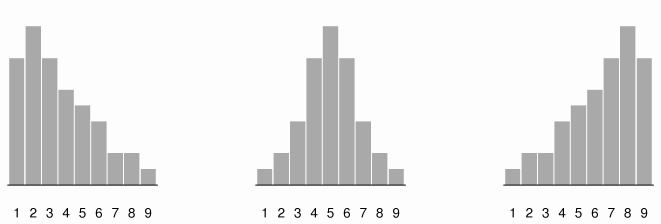
\includegraphics[scale=0.2]{Bilder/SymmetrieSchiefe.png}
\end{center}
 
\subsection{Lageregeln}
\begin{itemize}
\item Symmetrische und unimodale Verteilung
\[
\overline{x}\approx x_{med} \approx x_{mod}
\]
\item linksteile Verteilung
\[
\overline{x} > x_{med} > x_{mod}
\]
\item rechtssteile Verteilung
\[
\overline{x} < x_{med} < x_{mod}
\]
\item gruppierte Daten: auch für Histrogramme gültig
\end{itemize}

\subsection{Maßzahlen für Schiefe}
\subsubsection*{Quantilskoeffizient}
\[\resizebox{0.25\textwidth}{!}{$
g_p = \frac{(\tilde{x}_{1-p} - \tilde{x}_{med}) - (\tilde{x}_{med} - \tilde{x}_p) }{\tilde{x}_{1-p} - \tilde{x}_p} = 
\begin{cases}
g_p = 0 ~&\text{symmetrische Verteilung} \\
g_p > 0 ~&\text{linkssteile Verteilung} \\
g_p < 0 ~&\text{rechtsteile Verteilung} 
\end{cases}, ~0<p<0.5
$}
\]

$g_{0.25}$ ist Quartilskoeffizient
\subsubsection*{Momentenkoeffizient}
\[\resizebox{0.2\textwidth}{!}{$
g_m = \frac{m_3}{s_x^3}, ~ m_3=\frac{1}{n}\sum_{i=1}^n(x_i - \overline{x})^3 \Rightarrow 
g_m = \frac{1}{n}\sum_{i=1}^n\left(\frac{x_i-\overline{x}}{s_x}\right)^3 = 
\begin{cases}
g_m = 0 ~&\text{symmetrisch} \\
g_m > 0 ~&\text{linkssteil} \\
g_m < 0 ~&\text{rechtsteil} 
\end{cases}
$}
\]

\subsection{Wölbung und Extremwerte}
\begin{align*}
k &= \frac{m_4}{s_x^4} ~\text{mit}~ m4=\frac{1}{n}\sum_{i=1}^n(x_i - \overline{x})^4 \\
&= \frac{1}{n}\sum_{i=1}^n\left(\frac{x_i - \overline{x}}{s_x}\right)^4
\end{align*}

Exzess-Kurtosis: $k^\star = k-3$
\begin{itemize}
\item $k^\star \approx 0$: normalgipflig, mesokurtisch
\item $k^\star > 0 $: steilgipflig, leptokurtisch, stark ausprägter schmaler Gipfel, häufigere extreme Werte
\item $k^\star < 0$: flachgipflig, platykurtisch, seltenere extreme Werte
\end{itemize}

\subsection{Lorenzkurve}
\begin{itemize}
\item Punkt (0,0) immer in der Grafik enthalten
\item horizontale Achse in gleichen Längen
\[
u_j=\frac{j}{n}, ~j =1,...,n
\]
\item vertikale Achsen berechnen
\[
v_j = \frac{ \sum_{i=1}^jx_{(i)} }{ \sum_{i=1}^n x_{(i)} }, ~j=1,...,n
\]
\item $x=u_j$ und $y=v_j$ eintragen und verbinden
\item Lorenzkurve unterhalb der Winkelhalbierenden
\item streng monoton steigend und nächstes Polygonsegment gleich groß oder größer als zuvor
\end{itemize}

\subsection{Gini-Koeffizient (Lorenz'sche Konzentrationsmaß)}
\[
G = 2 \cdot F, ~\text{F Fläche zwischen Kurve und Diagonalen}
\]

\subsubsection*{Berechnung}
\begin{align*}
G &= \frac{ 2\sum_{i=1}^n i \cdot x_{(i)} -(n+1) \sum_{i=1}^nx_{(i)} }{n\sum_{i=1}^n x_{(i)}} \\
&= 1 - \frac{1}{n}\sum_{i=1}^n(v_{i-1}+v_i), ~0\leq G \leq \frac{n-1}{n}
\end{align*}

\subsubsection*{Normierter Gini}
\[
G^+ = \frac{n}{n-1}G, ~0 \leq G^+ \leq 1
\]
0 für keine Konzentration (Gleichverteilung) und 1 für vollständige Konzentration (Monopol)

\subsubsection*{Eigenschaften des Gini}
\begin{itemize}
\item unempfindlich gegen relatives Wachstum:$G^+$ unverändert, wenn x-Werte um selben Faktor wachsen/schrumpfen
\item empfindlich gegen Ausreißer am oberen Ende
\item verallgemeinerte Lorenzkurver und Gini-Koeffizient auf Merkmale mit negativen Ausprägungen anwendbar, Lorenz-Start nicht zwingend bei (0,0), Gini > 1 möglich
\end{itemize}

\subsection{Herfindahl-Index}
sagt dasselbe wie normierter Gini
\[
H:=\sum_{i=1}^np_i^2, ~p_i:=\frac{x_i}{\sum_{j=1}^nx_j}
\]
Wertebereich $x_i$: $\frac{1}{n}, 1$, identisch $x_i$ bis Monopol

%=========================================================================================================================================================================================================================

\section{Wichtige parametrische Verteilungen}

\subsection{Diskrete parametrische Verteilungen}
\subsubsection{Bernoulli-Verteilung}
Modelliert Experiment mit 2 mögl. Ausgängen (Münzwurf):
\begin{align*}
P(X=1) &= f(1) = \pi \\
P(X=0) &= f(0) = 1 - \pi, ~\pi \in [0,1] \\
X &\sim \mathcal{B}(\pi)
\end{align*}

\subsubsection{Diskrete Gleichverteilung}
alle Ausprägungen gleichwahrscheinlich, \\
endlicher Träger $T={x_1, x_2, ..., x_k}$:
\begin{align*}
P(X=x) = f(x)=\frac{1}{k}|(x_i \in T) \\
X \sim \mathcal{U}_D(a,b), ~ a,b \in \mathbb{N}
\end{align*}

\subsubsection{Geometrische Verteilung}
Modelliert Anzahl Versuche bis A zum erster Erfolg eintritt
\[
f(x)= \underbrace{(1 - \pi)^{x-1}}_{\text{(x-1)-mal } \overline{A}}
 \cdot \underbrace{\pi}_{\text{1-Mal A}}|(x \in T), \pi \in (0,1)
\]
\[
X \sim \mathcal{G}(\pi)
\]

\subsubsection{Binomialverteilung}
Modelliert Anzahl Erfolge mit fester Anzahl Versuchen
\[
P(X=x)=f(x)=\binom{n}{k} \cdot \pi^x(1-\pi)^{n-x}, ~ x \in T 
\]
\[
X \sim \mathcal{B}(n, \pi), ~ n \in \mathbb{N}, ~\pi \in [0,1]
\]

\subsubsection{Negative Binomialverteilung}
Verwendung: Wartezeiten/Misserfolge; "alle Fehlerfolge vor Erfolgen" \\
$T_X=\{n, n+1, n+2, ...\}$ mit $n \in \mathbb{N}^+, \pi \in (0,1)$
\[\resizebox{0.2\textwidth}{!}{$
f(x)=\binom{x-1}{n-1}\pi ^n(1-\pi)^{x-n}|(x \geq n), \pi \in (0,1), T_X=\{n, n+1, ...\} ~ n \in \mathbb{N}^+
$}
\]
\[
X \sim \mathcal{NB}(n, \pi)
\]

\subsubsection{Hypergeometrische Verteilung}
Modelliert Anzahl Erfolge markierter El. ohne Zurcklegen \\
Träger für hypergeo. Verteilung:
\[
T={max(0, n-(N-M)), ...,min(n,M)}
\]

\[
f(x)=\frac{\binom{M}{x} \binom{N-M}{n-x}}{\binom{N}{n}},~ x \in T
\]

\[
X \sim \mathcal{H}(n,N,M)
\]

Approximation der Verteilung:
\[
\mathcal{H}(n,N,M) \approx \mathcal{B}\left(n, \pi = \frac{M}{N}\right)
\]

\subsubsection{Poisson-Verteilung}
Modelliert Anzahl Ereignisse mit festen Zeit/Raumbereich $\rightarrow$ konstante Rate, unabhängig (Anzahl Anrufe Callcenter)
\[
f(x)=exp(-\lambda)\frac{\lambda^x}{x!}|(x \in T), t= \mathbb{N^+}
\]
\[
X \sim \mathcal{P}(\lambda)
\]

Approximation:
\[
\mathcal{B}(n, \pi) \approx \mathcal{P}(\lambda =n\pi)
\]

\subsection{Stetige parametrische Verteilungen}

\subsubsection{Stetige Gleichverteilung}
Modelliert kontinuierliche ZV, alle gleichwahrscheinlich (Auswahl eines Punkts auf Strecke von 0 bis 1)
Träger $T=[a,b] \in \mathbb{R}$
\[
f(x) = \begin{cases}
\frac{1}{b-a} &x\in [a,b] \\
0 &\text{sonst}
\end{cases}
\]
\[
X \sim \mathcal{U}[a,b]
\]

\subsubsection{Exponentialverteilung}
Modelliert die Zeit zw. 2 aufeinanderfolgenden Ereignissen in Poissoin-Prozess (Zeit zwischen 2 Anrufen Callcenter) \\
positiver Träger $T=\mathbb{R}_+^0$
\[
f(x)= \begin{cases}
\lambda exp(-\lambda x) &x \geq 0 \\
0 &\text{sonst}
\end{cases}
\]
\[
F(x)= \begin{cases}
1-exp(-\lambda x) &x\geq 0\\
0 &x<0
\end{cases}
\]

\[
X \sim \mathcal{E}(\lambda)
\]

\subsubsection{Gammaverteilung}
Verallgemeinert E-Verteilung und modelliert bit zum k-ten Ereignis in Poisson (Zeit bis 3 Kunden im Laden erscheinen)\\
positiver Träger $T=R_+$ und Parameter $\alpha , \beta \in \mathbb{R}_+$
\[
f(x) = \begin{cases}
\frac{\beta^{\alpha}}{\Gamma (\alpha)}x^{\alpha -1}exp{-\beta x} &x>0 \\
0 &\text{sonst}
\end{cases}
\]

Gammafunktion: $\Gamma(\alpha)= \int_0^{\infty}x^{\alpha -1}exp(-x)dx$ \\
$\Gamma (x+1)=x!$ für x = 0, 1 ,2, ...

\[
X \sim \mathcal{G}(\alpha , \beta)
\]

\begin{itemize}
\item $\alpha = 1$ ergibt Exponentialfunktion $\lambda = \beta$:$\mathcal{E}(\lambda)\equiv \mathcal{G}(\alpha =1, \beta = \lambda)$
\item $\alpha = \frac{d}{2} ~\text{mit}~ d \in \mathbb{N}, \beta = \frac{1}{2}$ ergibt $\chi^2$-Verteilung: $\chi^2(d) \equiv \mathcal{G}(\alpha = \frac{d}{2}, \beta = \frac{1}{2})$
\end{itemize}

\subsubsection{Normalverteilung}
modelliert kontinuierliche Werte um Mittelwert mit sym. Verteilung (Körpergröße, Gewicht) \\
Träger $T=\mathbb{R}$ mit Parametern $\mu \in \mathbb{R}, \sigma^2 \in \mathbb{R}_+$
\[
f(x)=\frac{1}{\sqrt{2 \pi \sigma^2}}exp\left(-\frac{1}{2}\frac{(x-\mu)^2}{\sigma^2}\right), x\in \mathbb{R}
\]
$\mu = 0$ und $\sigma^2 = 1$ ist standardnormalverteilt.
\[
X \sim \mathcal{N}(\mu , \sigma^2)
\]

\begin{itemize}
\item Verschieben und skalieren
\[
X \sim \mathcal{N}(\mu , \sigma^2) \Rightarrow (a+bX) \sim \mathcal{N}(a+b\mu ,b^2 \sigma^2)
\]
\item Summen und Differezen
\[
X_i \sim \mathcal{N}(\mu_i , \sigma^2_i) \Rightarrow \sum_i X_i \sim \mathcal{N}(\sum_i \mu_i , \sum_i \sigma^2_i)
\]
\item Integral der Normalverteilungsdichte nicht analytisch machbar
\end{itemize}

\subsubsection{Betaverteilung}
modelliert W.keiten/Anteile/Verhätlnisse aufgrund von Beobachtungen mit $\alpha$ Einfluss von Erfolgen, $\beta$ Einfluss Misserfolgen, Sicherheit über wahre Verhältnis \\
Träger $T=(0,1)$ und Parameter $\alpha , \beta \in \mathcal{R}_+$
\[
f(x)= \begin{cases}
\frac{1}{B(\alpha , \beta)}x^{\alpha - 1}(1-x)^{\beta -1} &0<x<1 \\
0 &\text{sonst}
\end{cases}
\]
Betafunktion:
\[
B(\alpha , \beta)= \frac{\Gamma(\alpha) \Gamma(\beta)}{\Gamma(\alpha + \beta)}=\int_0^1x^{\alpha-1}(1-x)^{\beta -1}dx
\]
Normierungseigenschaft:
\[
\int_0^1f(x)dx = 1
\]

\[
X \sim \mathcal{Be}(\alpha , \beta)
\]

\subsubsection{Cauchy-Verteilung}
modelliert Prozee mit starken Schwankungen (heavy tails)\\
Träger $T=\mathbb{R}$
\[
f(x) = \frac{1}{\pi} \cdot \frac{1}{1+x^2}
\]

\[
F(x)=\frac{1}{2}+\frac{\arctan(x)}{\pi}
\]

\[
X \sim \mathcal{C}
\]

\subsubsection{Dichtetransformationssatz}
Träger: $T_Y= g(T_X)=\{ y:(\exists x \in T_X : g(x)=y) \}$
\[
f_Y(y) = f_X(g^{-1}(y))\mid (g^{-1})'(y)\mid
\]

Formal: $X: \Omega \rightarrow T_X$ und $g:T_X \rightarrow T_Y$
\[
Y(\omega ) = (g \circ X)(\omega ) = g(X(\omega ))
\]

Nett to know

\begin{itemize}
\item $P(X \in [a,b])=P(Y=g(X) \in [g(a),g(b)])$ also $\int_a^bf_X(x)dx=\int_{g(a)}^{g(b)}f_Y(y)dy$
\item $(g^{-1})'(y)=\frac{1}{g'(g^{-1}(y))}$
\item $g(x): \mid g'(x)\mid \ll 1 \Leftrightarrow \mid g'(x)\mid \gg 1$ \\
flache Steigung, lange Intervalle $T_X$ zu kurzen Intervallen $T_Y$
\item $g(x): \mid g'(x)\mid \gg 1 \Leftrightarrow \mid g'(x)\mid \ll 1$ \\
steile Steigung, kurze Intervalle $T_X$ zu langen Intervallen $T_Y$
\end{itemize}

\subsubsection{Inversionsmethode}
\begin{enumerate}
\item Relisationen $u_1, ..., u_n$ erzeugen mit $U_i \sim \mathcal{U}[0,1]$
\item $x_i=F_X^{-1}(u_i),~i=1,...,n$ berechnen
\end{enumerate}

\[
f(x)=f_U(F_X(x))\cdot F'_X(x)=1 \cdot f_X(x)=f_X(x)
\]

%=========================================================================================================================================================================================================================

\section{ZVs und multivariate Verteilungen}

\subsection{Allgemeine Zufallsvektoren}
\begin{enumerate}
\item Wahrscheinlichkeits-/Dichtefunktion
\[
f_\textbf{X}(\textbf{x})=f_{X_1,...X_n}(\textbf{x}_1, ..., \textbf{x}_n)
\]
\item Verteilungsfunktion
\[
F_\textbf{X}(\textbf{x})=P(X_1 \leq \textbf{x}_1 \wedge ... \wedge X_n \leq \textbf{x}_n)
\]
\item Randverteilungen
\[ \resizebox{0.2\textwidth}{!}{$
f_{X_i}(x_i)=\begin{cases}
\sum_{\textbf{x}:\textbf{x}_i=x_i}f_\textbf{X}(\textbf{x}) &\text{diskret} \\
\int_{- \infty}^{+\infty} ... \int_{- \infty}^{+\infty} f_{\textbf{x}}(u_1, ..., u_{i-1}, x_i, u_{i+1}, ..., u_n) du_1 ...du_{i-1}du_{i+1}du_m &\text{stetig}
\end{cases}
$}
\]
\end{enumerate}

\subsection{Gemeinsame Verteilungsfunktion}
\[ \resizebox{0.2\textwidth}{!}{$
F_{X,Y}:=P(X \leq x \wedge Y \leq y) = (\{\omega \in \Omega : X(\omega) \leq x \wedge Y(\Omega) \leq y\}
$}
\]

\subsection{Gemeinsame Wahrscheinlichkeitsfunktion}
\begin{align*}
f_{X,Y}(x,y) &= P(X = x \wedge Y=y) \\
&= P(X=x, Y=y) ~~~\forall x \in T_X, y \in T_Y
\end{align*}

\[ 
F_{X,Y}(x,y)= \sum_{\{u: u \leq x \}} \sum_{\{v:v \leq y\}} f_{X,Y}(u,v)
\]

\subsection{Gemeinsame Dichtefunktion}
\[ \resizebox{0.2\textwidth}{!}{$
F_{X,Y}(x,y)=\int_{v= - \infty}^y \int_{u=- \infty}^x f_{X,Y}(u,v)dudv ~~~ \forall x,y \in \mathbb{R}
$}
\]

\begin{itemize}
\item gemeinsame Dichte überall stetig, wo f stetig
\[
\frac{\partial^2F(x,y)}{\partial x \partial y}=f(x,y)
\]
$\partial$ steht für Ableitung
\item normierte Dichtefunktion
\[
\int_{- \infty}^{+\infty} \int_{- \infty}^{+\infty} f(x,y)dxdy=1
\]
\item Wahrscheinlichkeiten für bel. Teilmengen $A \leqslant (\mathbb{R} \times \mathbb{R})$
\[
P((X,Y) \in A) = \int_A f(x,y)d(x,y)
\]
\end{itemize}

\subsection{Transformationsregel}
\[ \resizebox{0.25\textwidth}{!}{$
E(Z)=E(g(X,Y))= \begin{cases}
\sum_x \sum_y g(x,y)f_{X,Y}(x,y) &\text{X, Y diskret} \\
\int_{- \infty}^{+\infty} \int_{- \infty}^{+\infty} g(x,y)f_{X,Y}(x,y)dxdy &\text{X, Y stetig}
\end{cases}
$}
\]

\subsection{Randverteilungen}
\[
f_X(x)=\begin{cases}
\sum_{y \in T_Y} f_{X,Y}(x,y) &\text{X, Y diskret} \\
\int_{- \infty}^{+\infty} f_{X,Y}(x,y)dy &\text{X, Y stetig}
\end{cases}
\]
für $f_Y(y)$ andersherum

\subsection{Multinomialverteilung}
\[
f_X(x)=f_{X_1, X_2, X_3}(x_1,x_2,x_3)=\frac{n!}{x_1!x_2!x_3!}\pi^{x_1}\pi^{x_2}\pi^{x_3}
\]

$\mathcal{M}_{d}(n, \boldsymbol{\pi})$-verteilter Zufallsvektor $\boldsymbol{X}$
\[ \resizebox{0.18\textwidth}{!}{$
T_X=\{(x_1, x_2, ..., x_d): x_j \in {0,1, ...,n} \forall j \wedge \sum_{j=1}^dx_j=n\}
$}
\]
\[
\boldsymbol{\pi} = \{ \pi_1, ..., \pi_d), ~ \pi_j \in [0,1] \forall ~\text{und}~ \sum_{j=1}^d \pi_j=1
\]
\[
X_i \sim \mathcal{B}(n, \pi_i)
\]

\subsection{Unabhängige ZVs}
\begin{align*}
F_{X,Y}(x,y) &= F_X(x) \cdot F_Y(y) \\
f_{X,Y}(x,y)&=f_X(x) \cdot f_Y(y) \\
P(X=x,Y=y) &= P(X=x) \cdot P(Y=y)
\end{align*}

\subsection{Vektoren unabhängiger ZVs}
\[
f_{X_1, ..., X_n}(X_1 = x_1, ..., X_n= x_n)= \prod_{i=1}^nf_{X_i}(x_i)
\]

\[
P(\bigcap_i (X_i = x_i)= \prod_{i=1}^n P(X_i = x_i)
\]

\subsection{Faltung}
Für unabhängige ZV
\begin{align*}
P(X+Y = z) &= \sum_x f_X(x) \cdot f_Y(z-x)\\
		&= \sum_y f_X(z-y) \cdot f_Y(y)
\end{align*}

Stetige unabhängige X,Y:
\[
f_Z(z)=\int f_X(x)f_Y(z-x)dx = \int f_X(z-y)f_Y(y)dy
\]

\subsubsection*{Bedingte Verteilung diskreter ZV}
\begin{align*}
F_{X|Y}(x|y) &= P(X \leq x | Y=y) = \frac{P(X \leq x, Y =y)}{P(Y=y)} \\
f_{X|Y}(x|y) &= P(X =x | Y=y) = \frac{P(X=x, Y=y)}{P(Y=y)} \\
&= \frac{f_{X|Y}(x,y)}{f_Y(y)}
\end{align*}

\subsection{Bedingte Verteilung stetiger ZV}
\begin{align*}
F_{X|Y}(x,y) &:= \int_{- \infty}^x\frac{f_{X,Y}(u,y)}{f_Y(y)}du, f_Y(y) > 0 \\
f_{X|Y}(x|y) &:= \frac{f_{X,Y}(x,y)}{f_Y(y)}
\end{align*}

\textcolor{gray}{\subsection{Bedingte Momente}
\[
E(X|Z=z) := \begin{cases}
\sum_{X \in T_X} xP(X=x|Z=z) ~ \text{X diskret} \\
\int_{- \infty}^{\infty}xf_{X|Z}(x|Z=z)x ~ \text{X stetig}
\end{cases}
\]
}

\textcolor{gray}{
\begin{align*}
Var(X|Z=z) :&= E[(X-E(X|Z=z))^2|Z=z] \\
&= \begin{cases}
\sum_{x \in T_X}(x-E(X|Z=z))^2P(X=x|Z=z) ~ \text{X diskret} \\
\int_{-\infty}^{\infty}(x-E(X|Z=z))^2f_{X|Z}(x|Z=z)dx ~ \text{X stetig}
\end{cases}
\end{align*}
}

\subsection{Satz von iteriertem Erwartungswert}
\[
E(E(g(X)|Z)) = E(g(X))
\] 

\subsection{Satz von der totalen Varianz}
\[
Var(X) = E(Var(X|Z))+Var(E(X|Z))
\]

%=========================================================================================================================================================================================================================

\section{Schätzung und Grenzwertsätze}

\subsection{Gesetz großer Zahlen}
\[
E(\overline{X}_n) = \mu_X ,~~ Var(\overline{X}_n)= \frac{1}{n} \sigma_X^2 \xrightarrow{n \to \infty} 0
\]
\[
P(\mid \overline{X}_n - \mu_X \mid \geq \varepsilon) \xrightarrow{n \to \infty} 0 \forall \varepsilon > 0, ~~ \overline{X}_n \xrightarrow{P} \mu_X
\]

\subsection{Fundamentalsatz der Statistik (Glivenko-Cantelli)}
\[
P\left(\sup_{x \in \mathbb{R}}(\mid F_n(x) - F_X(x) \mid ) < \varepsilon\right) \xrightarrow{n \to \infty} 1, ~ \forall \varepsilon > 0 \forall x
\]

\subsection{Standadisierte ZV}
\begin{align*}
\tilde{X} &= \frac{X- \mu_X}{\sigma_X} \\
E(\tilde{X}) &= (E(X)-\mu_X)=0 \\
Var(\tilde{X})&=\frac{1}{\sigma^2_X}Var(X) = 1
\end{align*}

Standadisierung summierter ZVn:
\begin{align*}
E(Y_n) = n \cdot \mu_X, ~ Var(Y_n)= n \cdot \sigma_X^2 \\
Z_n = \frac{Y_n - n\mu_X}{\sqrt{n}\sigma_X}=\frac{1}{\sqrt{n}}\sum_{i=1}^n \frac{X_i-\mu_X}{\sigma_X}
\end{align*}

\subsection{Zentraler Grenzwertsatz}
\[
F_n(z) \xrightarrow{n \to \infty} F_{N(0,1)}(z) ~ \forall z \in \mathcal{R}
\]
\[
Z_n \sim \mathcal{N}(\mu = 0, \sigma^2 = 1) ~ \text{a :$\cong$ asymptotisch}
\]

Standadisierung:
\[
Y_n \sim \mathcal{N}(\mu = n\mu_X, \sigma^2= n \sigma_X^2)
\]

Speziell:
\[
\overline{X}_n \sim \mathcal{N}(\mu = \mu_X, \sigma^2=\frac{\sigma_X^2}{n}
\]

%=========================================================================================================================================================================================================================

\section{Zusammenhangsmaße metrischer Merkmale}

\subsection{Kovarianz}
\[
s_{xy} = \frac{1}{n-1} \sum_{i=1}^n(x_i - \overline{x})(y_i - \overline{y})
\]

\subsection{Bravais-Pearson-Korrelationskoeffizient}
\begin{align*}
r_{xy} &= \frac{1}{n-1}\sum_{i=1}^n \frac{(x_i - \overline{x})}{s_x} \frac{(y_i - \overline{y})}{s_y} \\
&= \frac{\sum_{i=1}^n(x_i - \overline{x})(y_i - \overline{y})}{\sqrt{\sum_{i=1}^n(x_i - \overline{x})^2 \sum_{i=1}^n(y_i - \overline{y})^2}} = \frac{s_{xy}}{s_xs_y}
\end{align*}

\begin{itemize}
\item $r_{xy}>0$: pos. Korrelation, linearer Zusammenhang
\item $r_{xy}<0$: neg. Korrelation, linearer Zusammenhang
\item $r_{xy}=0$: keine Korrelation, kein linearer Zusammenhang 
\end{itemize}

\subsubsection*{Lineare Transformation}
\begin{align*}
\tilde{r}_{xy}=r_{xy} &\Leftrightarrow a_X, a_Y ~\text{gleiches Vorzeichen} \\
\tilde{r}_{xy}=-r_{xy} &\Leftrightarrow a_X,a_Y ~\text{verschiedene Vorzeichen}
\end{align*}

\subsection{Kovarianz- und Korrelationsmatrix}
Beispielmatrix:
\[
\begin{pmatrix}
1 & r_{xy} & r_{xz} \\
r_{xy} & 1 & r_{yz} \\
r_{xz} & r_{yz} & 1
\end{pmatrix}
\]

\subsection{Kovarianz ZV}
\[
Cov(X,Y)=E[(X-E(X))(Y-E(Y))]
\]

\subsubsection{Verschiebungssatz Kovarianz}
\[
Cov(X,Y)=E(XY)-E(X)E(Y)
\]

\subsubsection{Lineare Transformation}
\begin{align*}
Cov(a+bX,c+dY)&=b\cdot d \cdot Cov(X,Y)\\
\rho(a+bX, c+dY) &= \rho(X,Y)
\end{align*}

\subsection{Korrelation ZV}
\[
\rho(X,Y)=\frac{Cov(X,Y)}{\sqrt{Var(X)}\sqrt{Var(Y)}}
\]

\[-1 \leq \rho(X,Y) \leq 1\]

\subsubsection{Unkorreliertheit}
Aus Unabhängigkeit folgt Unkorreliertheit, aber nicht andersrum
\[
E(XY)=E(X)E(Y) ~ \Rightarrow ~ Cov(X,Y)=0,~ \rho(X,Y)=0
\]

\subsubsection{Varianz der Summe zweier ZV}
\[
Var(X+Y)=Var(X)+Var(Y)+2\cdot Cov(X,Y)
\]

Wenn X und Y unabhängig und damit unkorreliert:
\[
Var(X+Y)=Var(X)+Var(Y)
\]

\subsection{Bivariate Standardnormalverteilung}
Parameter $\rho(\rho<1)$ und Träger $T=\mathbb{R}\times\mathbb{R}$

\[
f(x,y)=\frac{1}{2\pi \sqrt{(1-\rho^2)}}exp(-\frac{1}{2(1-\rho^2)}(x^2-2\rho xy+y^2)
\]

\subsection{Multivariate Normalverteilung}
\begin{align*}
\sigma_{XY} &:=Cov(X,Y)=\rho\sigma_X\sigma_Y \\
(X,Y) &\sim \mathcal{N}_2\left(\mu = (\mu_X, \mu_Y)^T, \Sigma= \begin{pmatrix}
\sigma_X^2 & \sigma_{XY} \\
\sigma_{XY} & \sigma_Y^2
\end{pmatrix}\right) \\
X &= (X_1, X_2, ..., X_d)^T \sim \mathcal{N}_d(\mu, \Sigma) \\
\Rightarrow f(x)&=\frac{1}{\sqrt{(2\pi)^d\mid \Sigma \mid}}exp\left(-\frac{1}{2}(x-\mu)^T\Sigma^{-1}(x-\mu) \right)
\end{align*}

\subsection{Spearman-/Rang-Korrelationskoeffizient}
X,Y (min.) ordinal:
\[
r_{xy}^{SP}=\frac{\sum(rg(x_i)-\overline{rg}_X)(rg(y_i)-\overline{rg}_Y)}{\sqrt{\sum(rg(x_i)-\overline{rg}_X)^2\sum(rg(y_i)-\overline{rg}_Y)^2}},~ -1 \leq r_{xy}^{SP} \leq 1
\]

\begin{itemize}
\item $r_{xy}^{SP} > 0$: gleichsinniger monotoner Zsmhang, x groß/klein $\rightarrow$ y groß/klein
\item $r_{xy}^{SP} < 0$: gleichsinniger monotoner Zsmhang, x groß/klein $\rightarrow$ y klein/groß
\item $r_{xy}^{SP} \approx 0$: kein monotoner Zsmhang
\end{itemize}

\subsubsection*{Monotone Transformation}
g und h streng monoton:
\[
\tilde{X}=g(X), ~ \tilde{Y}=h(Y)
\]

\begin{itemize}
\item beide monoton wachsend oder fallend
\[
r^{SP}(\tilde{X}, \tilde{Y})=r^{SP}(X,Y)
\]
\item nicht beide wachsend oder fallend
\[
r^{SP}(\tilde{X}, \tilde{Y})=-r^{SP}(X,Y)
\]
\end{itemize}

\subsection{Paarvergleichsmaße: Kendall's Tau}
\begin{itemize}
\item konkordant: Rangfolge $X = Y$, $x_i < x_j$ und $y_i < y_j$ oder $x_i > x_j$ und $y_i > y_j$
\item diskordant: Rangfolge $X \neq Y$, $x_i < x_j$ und $y_i > y_j$ oder $x_i > x_j$ und $y_i < y_j$ 
\end{itemize}

\[
\tau_{XY}= \frac{N_C-N_D}{n(n-1)/2}, ~N_C(\text{konkordante Paare}), ~N_D(\text{diskordante Paare})
\]

$\tau_{XY}$ betragsmäßig kleiner $r_{XY}^{SP}$

\subsubsection{Goodman-Kruskal}
ignoriert Paare mit Bindungen
\[
\gamma_{XY}=\frac{N_C-N_D}{N_C+N_D}
\]

\subsubsection{Somers' D}
Y binär:
\[
D := \frac{N_C-N_D}{\text{Anzahl Paare mit ungleichem Y}}
\]

\subsection{ROC-Kurve}
\begin{itemize}
\item $Y \in {0,1}$ dichotom (binär), $X$ min. ordinal skaliert
\item $TPR(c)$ = TruePositiveRate = Sensitivität = $f(\hat{Y}=1|Y=1)=f(X\geq c|Y=1)$
\item $FPR(c)$ = FalsePositiveRate = $f(\hat{Y}=1|Y=0)=f(X\geq c|Y=0)$
\item $TNR(c)$ = Spezifität = $f(\hat{Y}=0|Y=0)=1-f(X\geq c|Y=0)=1-FPR(c)$
\item ROC-Kurve verbindet Punkte $(FPR(c), TPR(c))$
\item Schwellenwert $c = [x_{(1)}, x_{(n)}]$, komischer Trennstrich
\item $c<x_{(1)}$: immer positiv, $\hat{y}_i=1 \forall i \Rightarrow (FPR(c),TPR(c))=(1,1)$
\item $c>x_{(n)}$: immer negativ, $\hat{y}_i=0 \forall i \Rightarrow (FPR(c),TPR(c))=(0,0)$
\item alle TPR/TNR für versch. c berechnen und ab in die Olga
\item x-Achse: FPR oder 1-TNR
\item y-Achse: TPR
\end{itemize}

\subsection{AUC}
Fläche unter ROC-Kurve
\[
AUC := \frac{N_C+N_E/2}{n}
\]
$N_E$: Anzahl Paare mit Bindungen in X, $N$ Anzahl Paare mit unterschiedlichem Y

\begin{itemize}
\item perfekte Trennbarkeit mit AUC-Wert von 1
\item Unabhängigkeit von X und Y mit Wert von ca. 0,5
\item behandelt Sensitivität und Spezifität gleich
\item positiver prädikativer Wert (ppV): $f(Y=1|\hat{Y}=1)$
\item negativer prädikativer Wert (npV): $f(Y=0|\hat{Y}=0)$
\end{itemize}

\[
ppV := \frac{TP}{TP + FP}, ~npV:= \frac{TN}{TN + FN}
\]

%=========================================================================================================================================================================================================================

\section{Kausalität und Korrelation}

\subsection{Kausale und assoziative Strukturen}
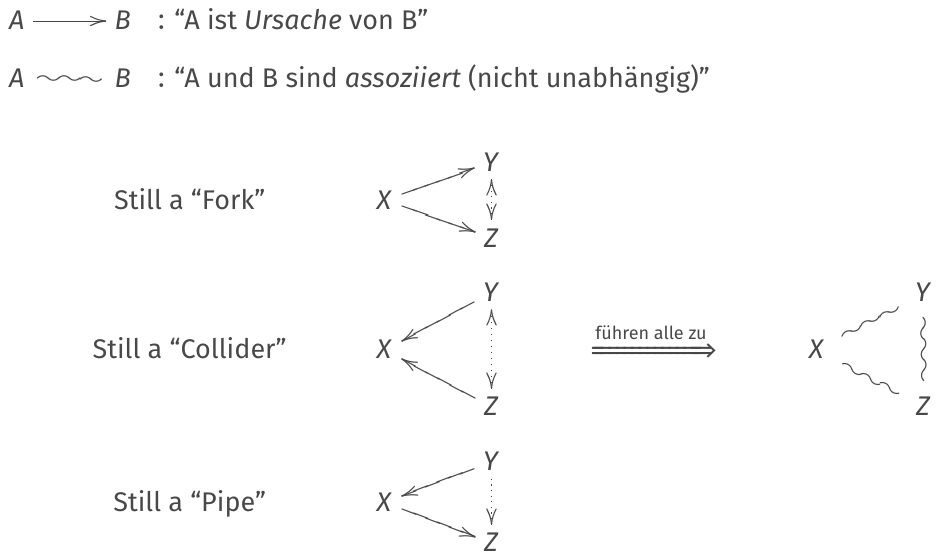
\includegraphics[scale=0.2]{Bilder/kasualassostruk.png} 
\begin{itemize}
\item unterschiedliche kausale Strukturen egeben identische assozitive
\item Vorsicht bei (kausaler) Interpretation
\item kausal stochastisch/probabilistisch gemeint
\end{itemize}

\subsection{Confounding}
\begin{itemize}
\item gemeinsame Ursache X für Variablen Y, Z (Fork)
\item erzeugt oft marginale Abhängigkeiten zw. nicht kausal verbundenen Y und Z (Scheinkorrelation/ spurious correlation)
\item kann auch evtl. vorhandene (bedingte) Assoziationen abschwächen oder umkehren (Simpson's Paradox)
\end{itemize}

\subsection{Simpson's Paradox}
\begin{itemize}
\item beschreibt häufig auftretendes Phänomen
\item Durch Bedingen auf Drittvariablen können Assoziationen entstehen, verschwinden oder Richtung ändern
\item Synonym: omitted variable bias
\end{itemize}

\subsection{Conditioning on the Collider}
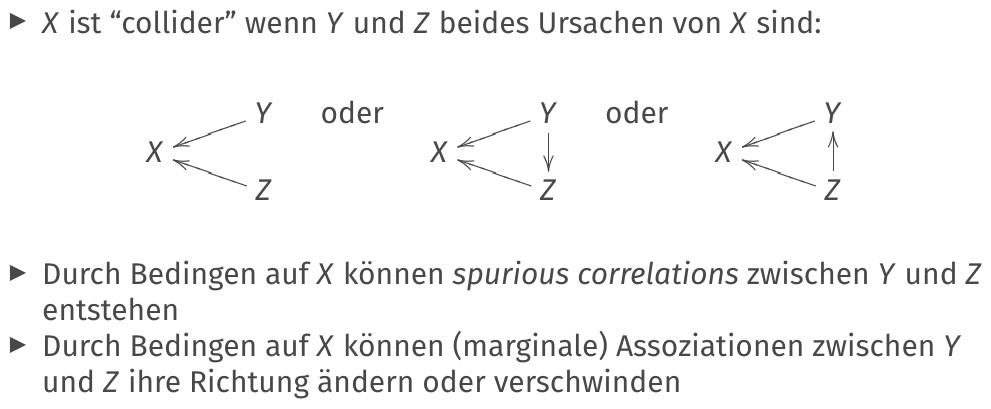
\includegraphics[scale=0.2]{Bilder/on the collider.png}

\subsubsection*{endogenous selection bias}
Ob Untersuchungseinheit in beobachteter Stichprobe abhängig von Variable abhängig, die von untersuchten Variablen abhängig ist $\Rightarrow$ selection-distortion effect

%=========================================================================================================================================================================================================================

\includepdf{Verteilungen.pdf} 

\end{multicols}
\end{document} 
